\documentclass{article}
\usepackage{amsmath}   % for mathematical equations
\usepackage{graphicx}  % for including graphs and images
\usepackage{float}     % to force figure placement
\usepackage{caption}   % for figure captions
\usepackage{siunitx}   % for units formatting
\usepackage{hyperref}  % for links

\title{Lab Report 1: Lab 1 - 3}
\author{Enrique Rivera Jr \\ Marcus}
\date{\today}

\begin{document}
\maketitle

\begin{center}
\section*{Lab 1: Basic Measurements and Oscilloscope Use}
\end{center}

\section{Introduction}
This lab introduces basic electronic measurement techniques using a multimeter and oscilloscope. 
The objective is to measure DC and AC voltages, understand the concept of output impedance, and 
analyze waveforms using a function generator. By constructing simple circuits, we will learn 
how to measure voltage, current, and impedance, and observe the behavior of waveforms under 
different conditions.

\section{Methods / Notes}
    \subsection{Breadboard Layout and Measurement}
    Using a multimeter in buzzer mode, we first determined the internal connections of a 
    breadboard. The multimeter's buzzing feature was used to identify connected holes.

    \begin{figure}[H]
        \centering
        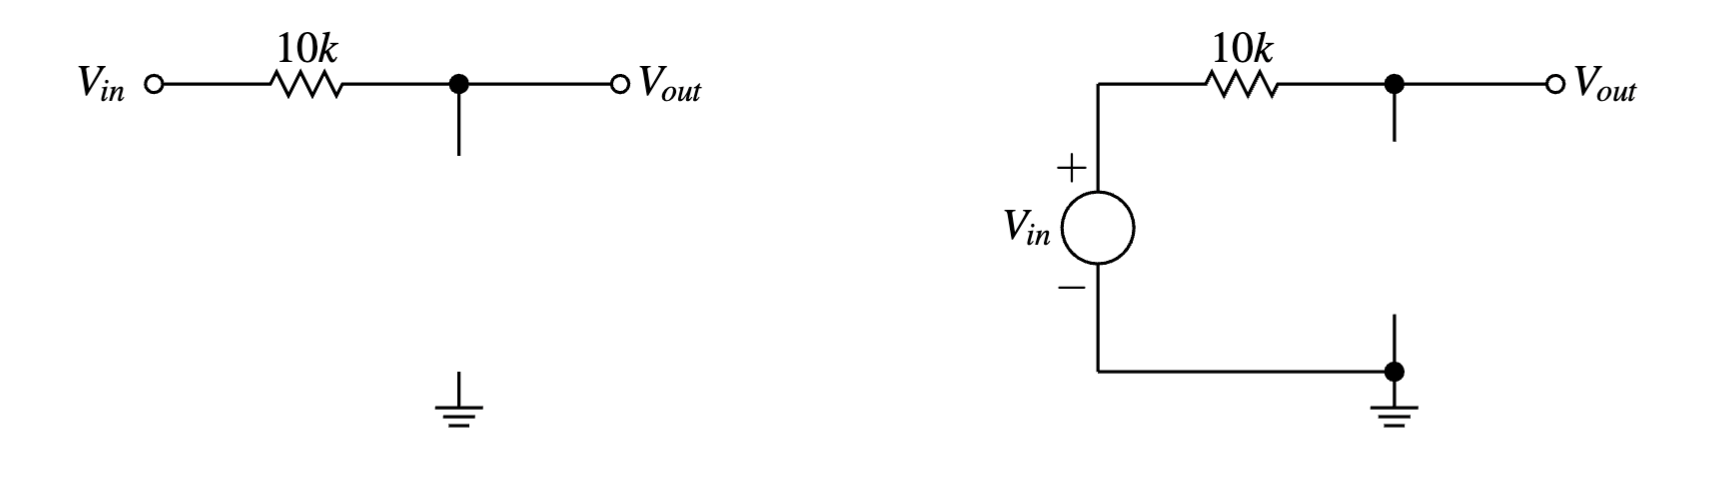
\includegraphics[width=0.8\textwidth]{img/other/Open_Circuit.png} % Replace with actual image path
        \caption{Open Circuit}
        \label{fig:opencircuit}
    \end{figure}

    \begin{figure}[H]
        \centering
        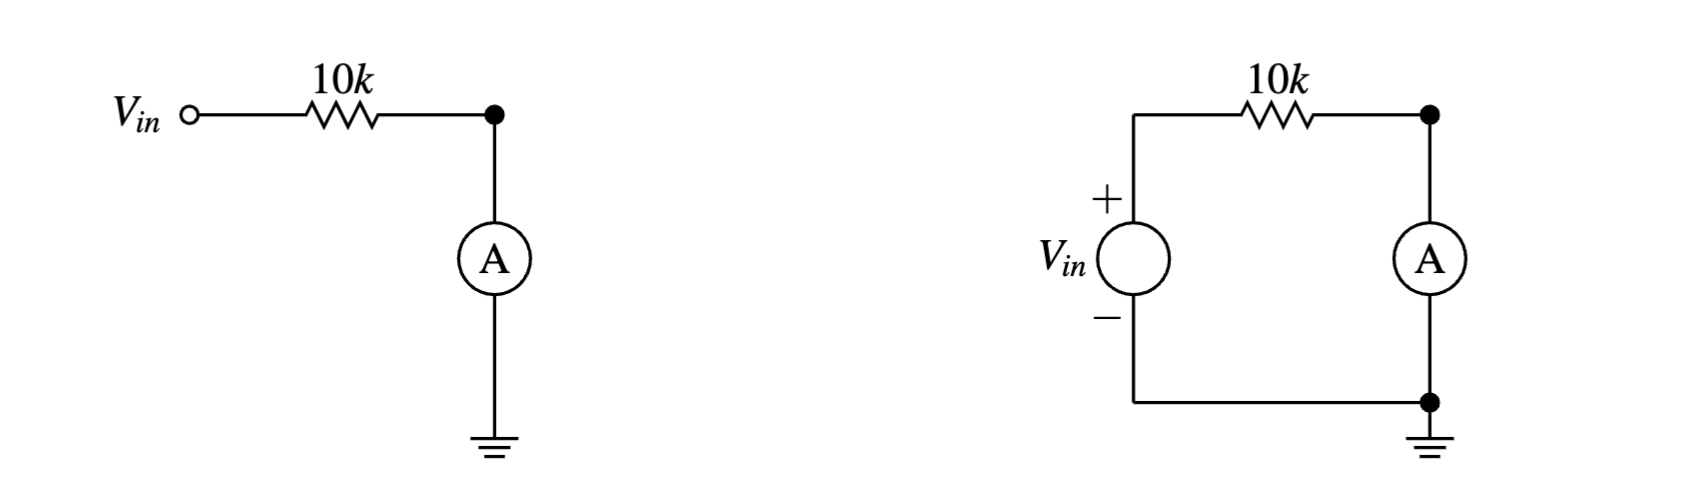
\includegraphics[width=0.8\textwidth]{img/other/Close_Circuit.png} % Replace with actual image path
        \caption{Closed Circuit}
        \label{fig:closedcircuit}
    \end{figure}

\subsubsection{Open and Closed Circuit Measurements}
The open circuit was constructed as shown in Figure \ref{fig:opencircuit}. The DC power supply 
was set to 5V, and the voltage was measured across the open circuit using the multimeter. Next, a c
losed circuit was constructed, and the current was measured using the ammeter function.


The output impedance $Z_{out}$ was calculated using the formula:
\[
Z_{out} = \frac{V_{\text{open}}}{I_{\text{closed}}}
\]

\subsubsection{Voltage Divider}
A voltage divider was constructed using two resistors of equal value (10k$\Omega$ each), and the output voltage was measured across the second resistor. The theoretical voltage was calculated using the voltage divider formula:
\[
V_{out} = V_{in} \times \frac{R_2}{R_1 + R_2}
\]

Both the measured and calculated voltages were recorded.

\subsubsection{Function Generator and Oscilloscope}
The output of a function generator was connected to an oscilloscope. 
A 1kHz sine wave with 2V peak-to-peak was generated. The waveform was observed and 
recorded on the oscilloscope screen. The effect of adding a 50$\Omega$ terminator was 
noted, and both the terminated and unterminated waveforms were sketched and compared.

\subsection{Results}
    \subsubsection{(1) Breadboard Layout}
    The following diagram shows the internal connections of the breadboard. The multimeter was used 
    to map out which holes were connected.

    \begin{figure}[H]
        \centering
        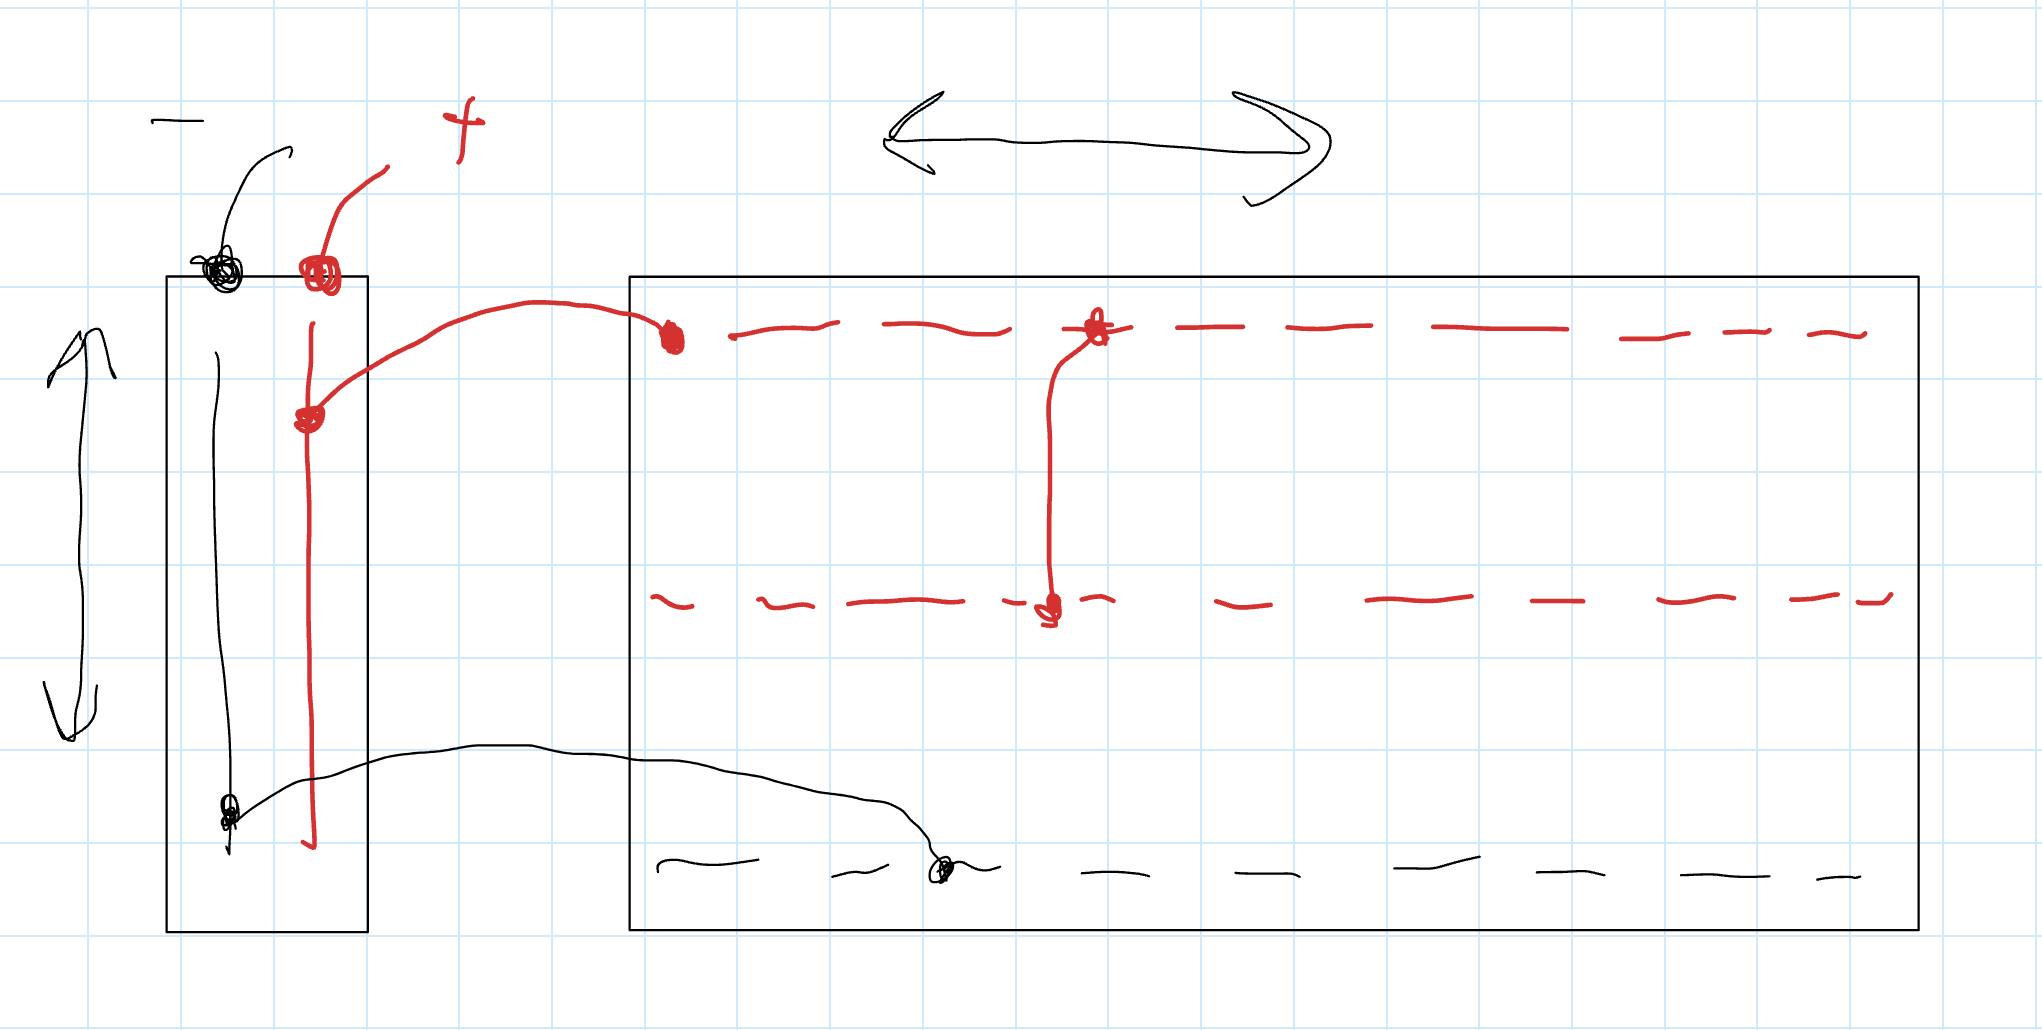
\includegraphics[width=0.8\textwidth]{img/Lab1_1.png} % Replace with actual image path
        \caption{How a breadboard`s internal connections are laid out.}
        \label{fig:breadboard_layout}
    \end{figure}


    \subsubsection{(2c) Open and Closed Circuit Measurements}
    The measured open circuit voltage was \SI{5}{V} and the closed circuit current was \SI{0.5}{A}. Using these values, the output impedance was calculated to be:
    \[
    Z_{out} = \frac{5 \text{V}}{0.5 \text{A}} = 10 \, \Omega
    \]

    \subsubsection{(3) Voltage Divider Results}
    The measured output voltage for the voltage divider was \SI{2.5}{V}, matching the theoretical calculation.

    \begin{table}[H]
    \centering
    \caption{Voltage Divider Results}
    \begin{tabular}{|c|c|c|}
    \hline
    $V_{in}$ (V) & $V_{out}$ (Measured) (V) & $V_{out}$ (Calculated) (V) \\ \hline
    5            & 2.5                      & 2.5                        \\ \hline
    \end{tabular}
    \end{table}

    \subsubsection{(4) Voltage Divider Cases}
    The following cases were considered for the voltage divider. When R2 $\gg$ R1, the output voltage is 
    approximately equal to the input voltage. When R2 $\ll$ R1, the output voltage is approximately zero.

    \begin{figure}[H]
        \centering
        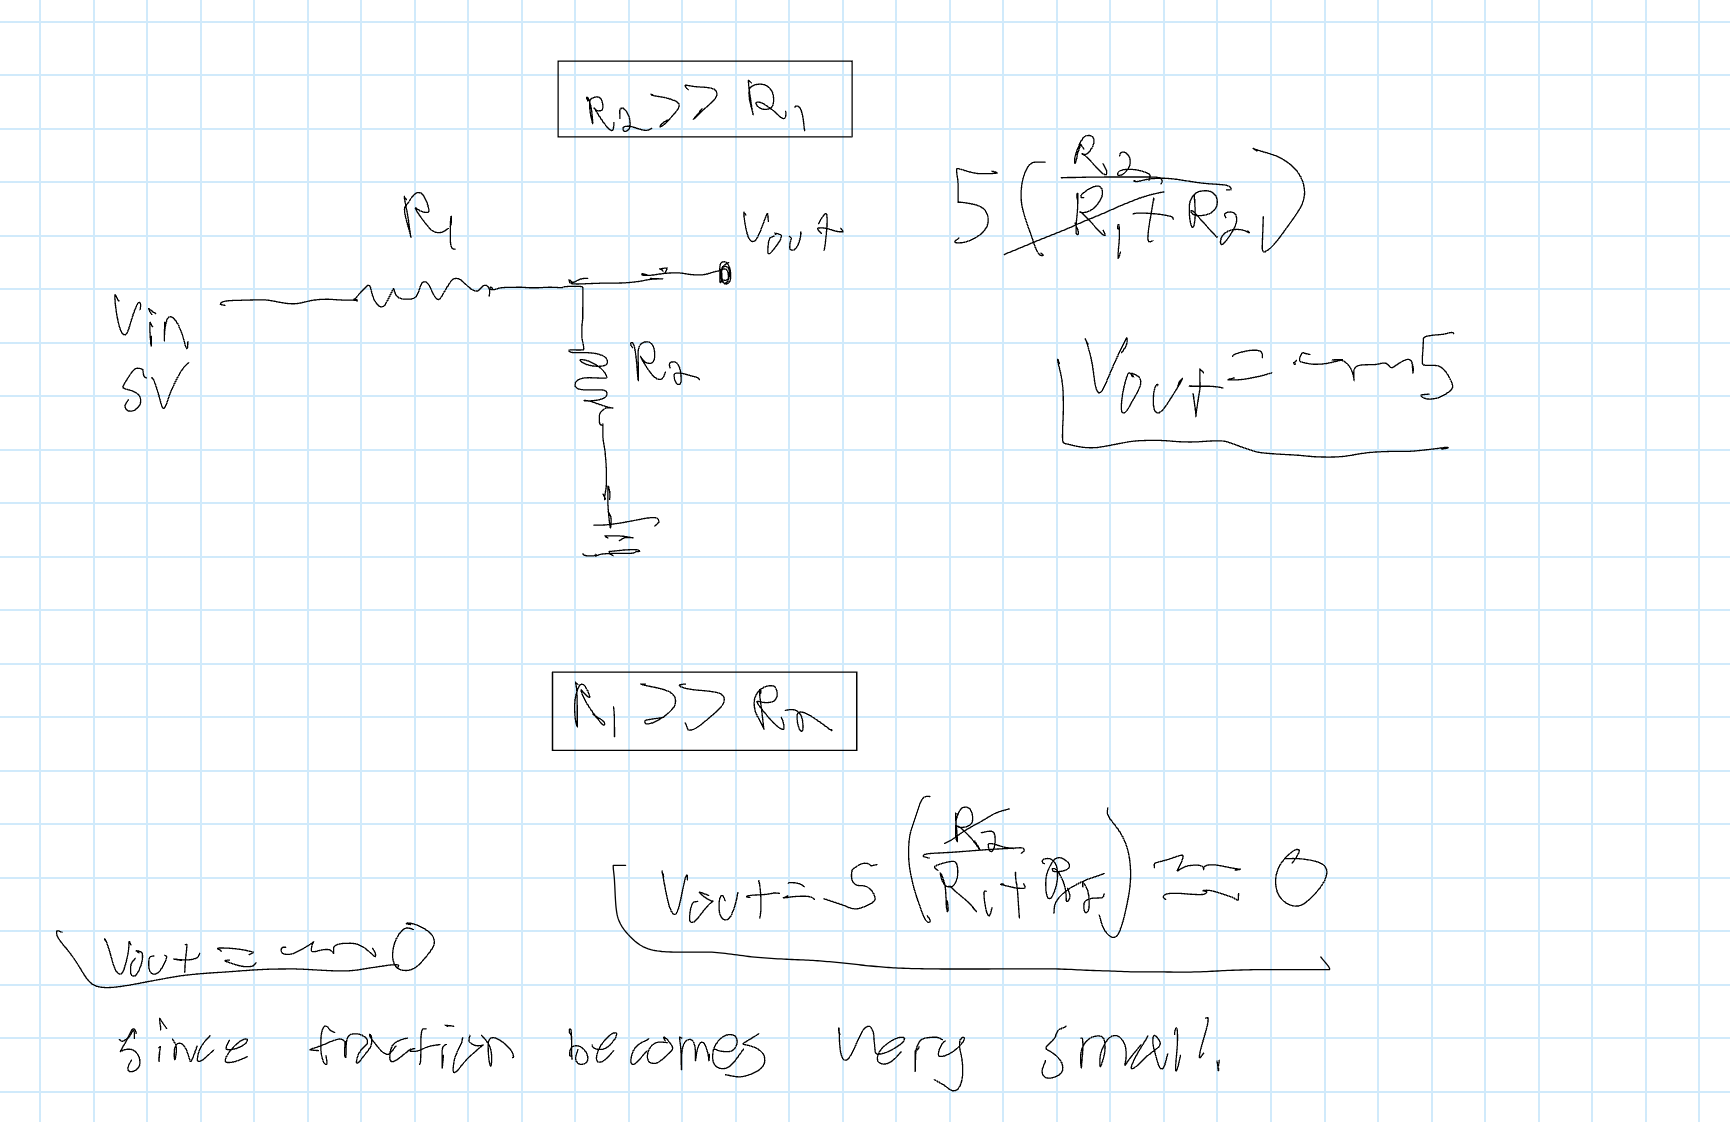
\includegraphics[width=0.9\textwidth]{img/Lab1_4.png}  % Replace with actual path
        \caption{Voltage Divider Cases}
        \label{fig:voltage_divider_cases}
    \end{figure}

    \subsubsection{(5) Function Generator and Oscilloscope}
    The following waveforms were observed using the oscilloscope for the function generator output.

    \begin{figure}[H]
        \centering
        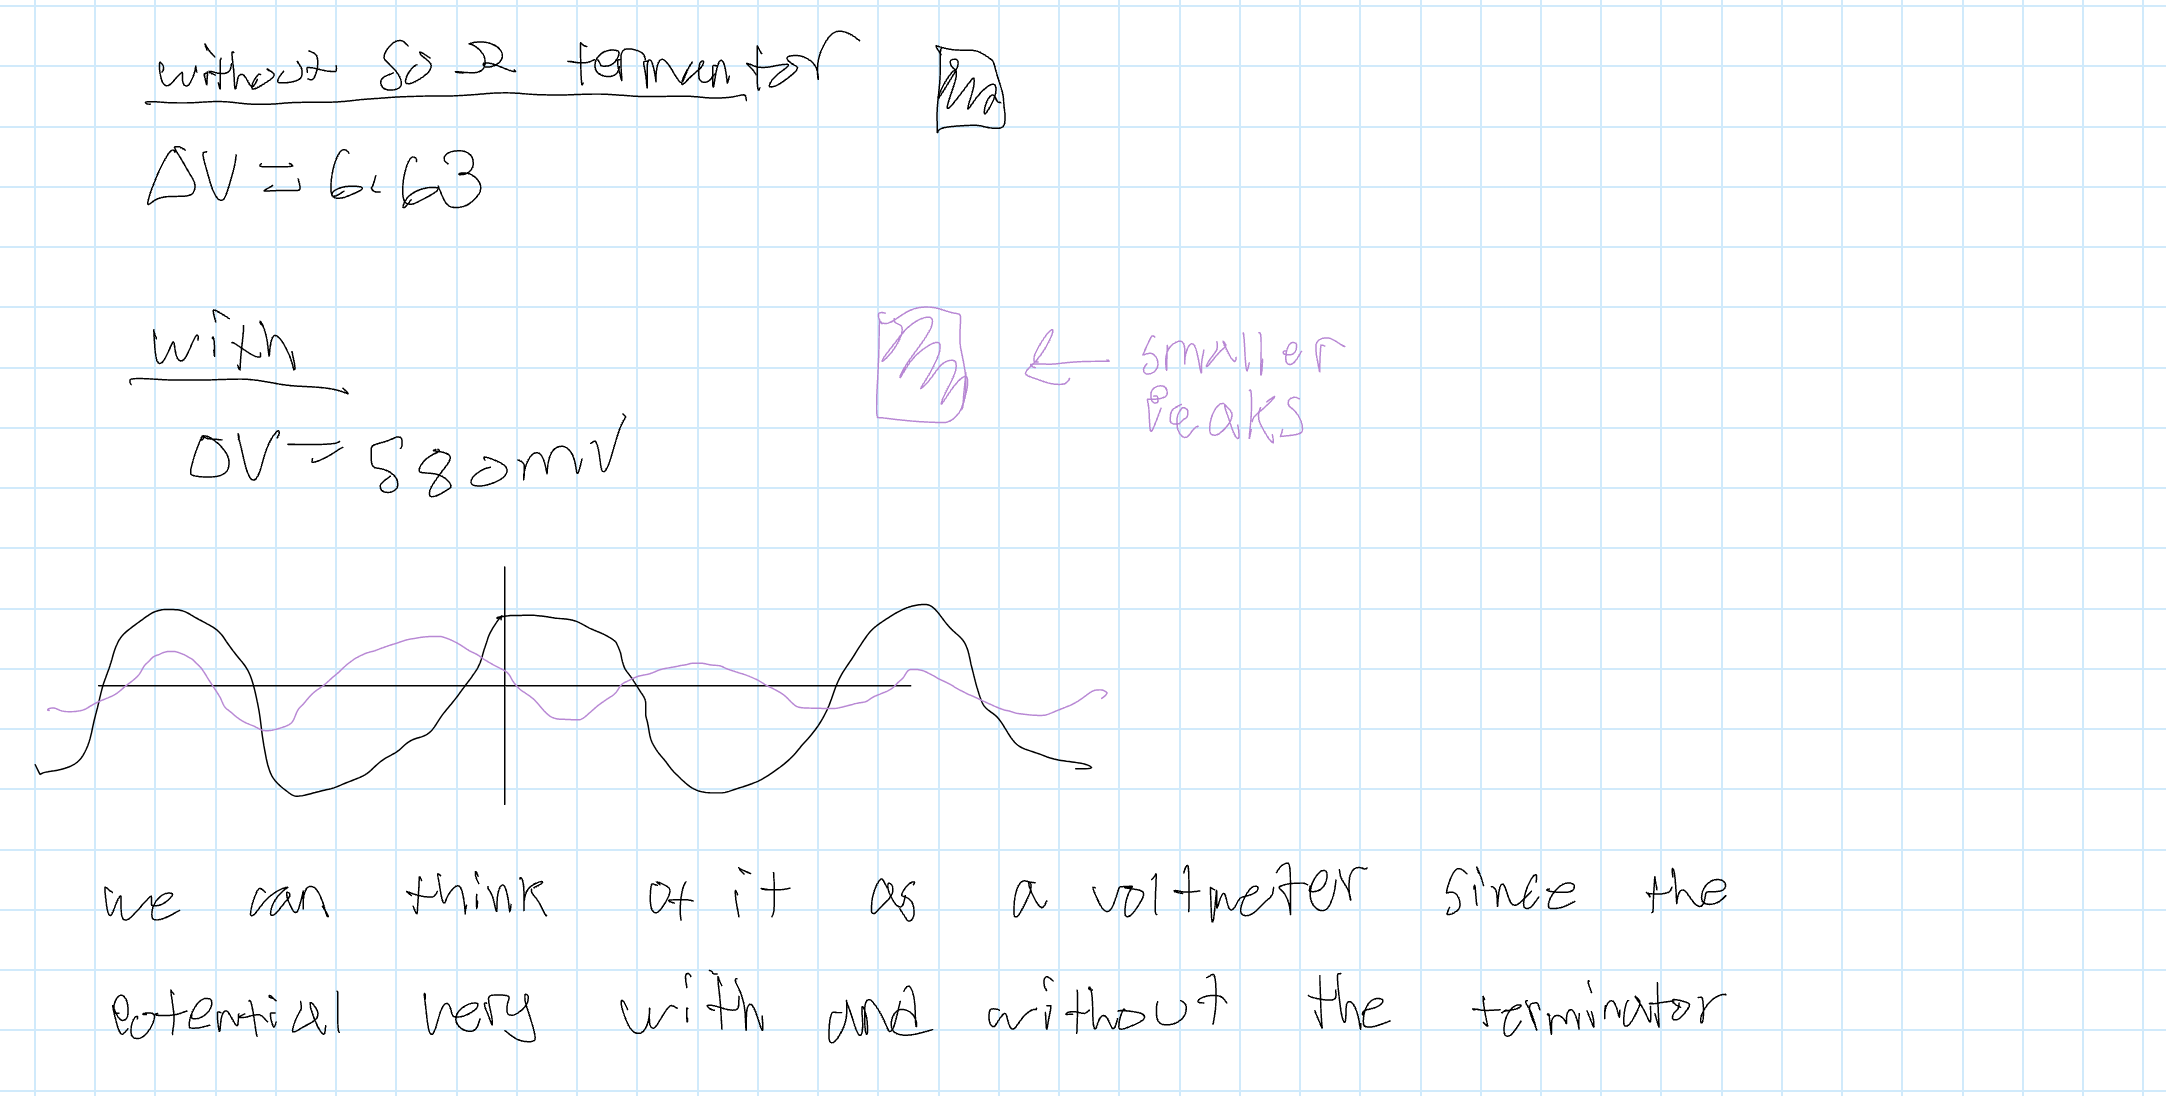
\includegraphics[width=0.9\textwidth]{img/Lab1_5.png}  % Replace with actual path
        \caption{Waveform with terminator connected and disconnected.}
        \label{fig:terminated_waveform}
    \end{figure}

    \subsubsection{(6) Trigger Effect}
    The trigger effect was observed by adjusting the trigger level and observing the waveform on the oscilloscope. 
    
    \begin{figure}[H]
        \centering
        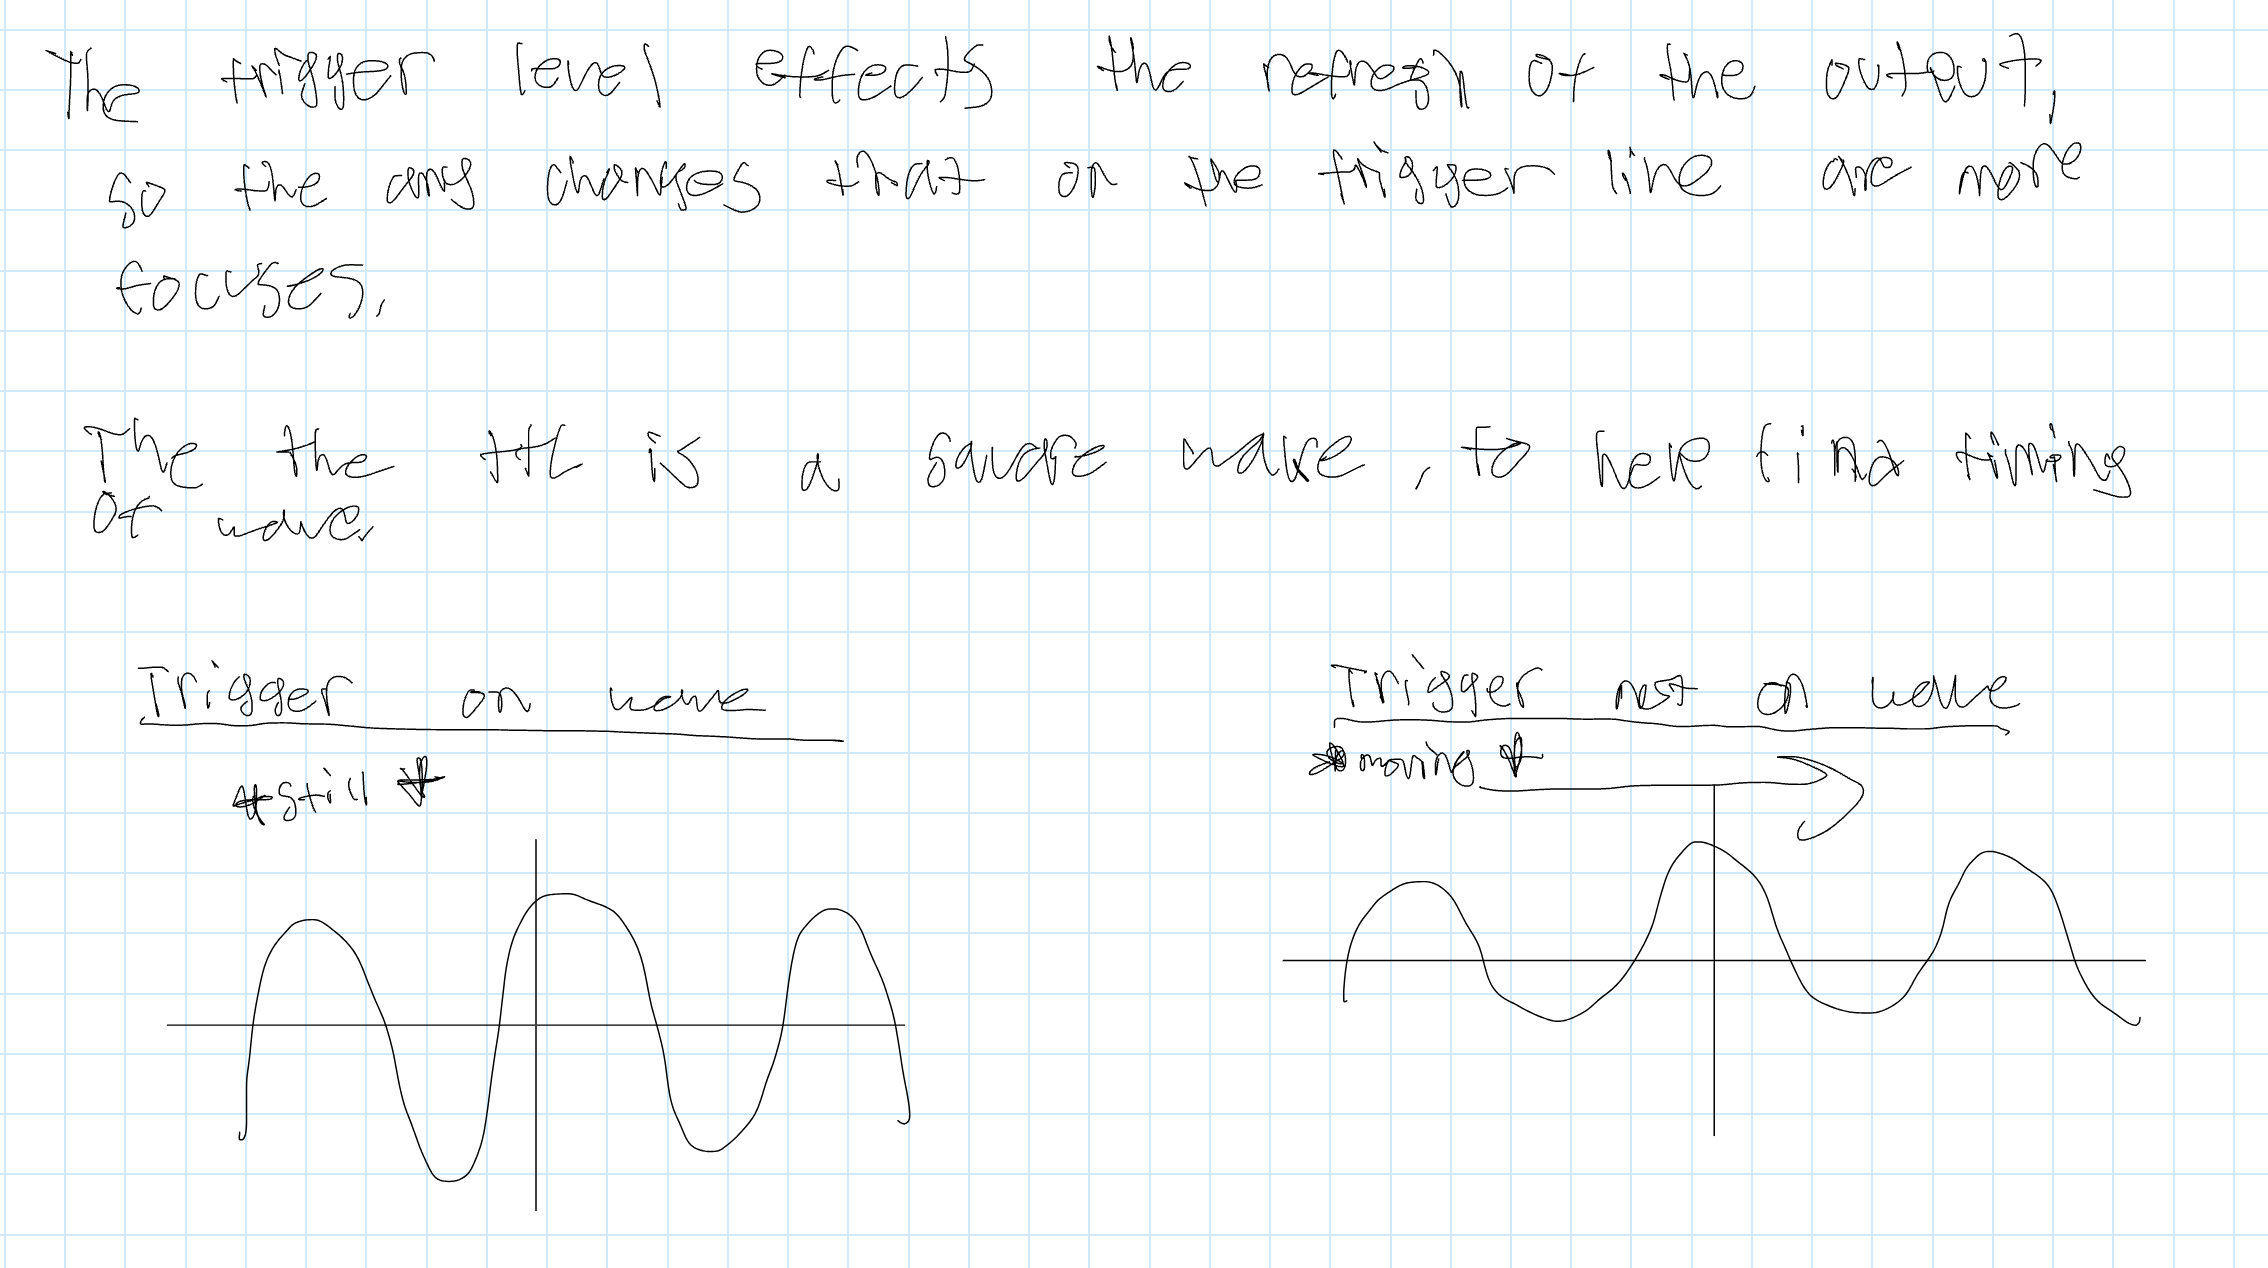
\includegraphics[width=0.9\textwidth]{img/Lab1_6.png}  
        \caption{Waveform with Trigger Level adjusted.}
        \label{fig:trigger_waveform}
    \end{figure}

    \subsubsection{(7) DC Offset Effect}
    The DC offset effect was observed by adjusting the DC offset and observing the waveform on the oscilloscope. 
    
    \begin{figure}[H]
        \centering
        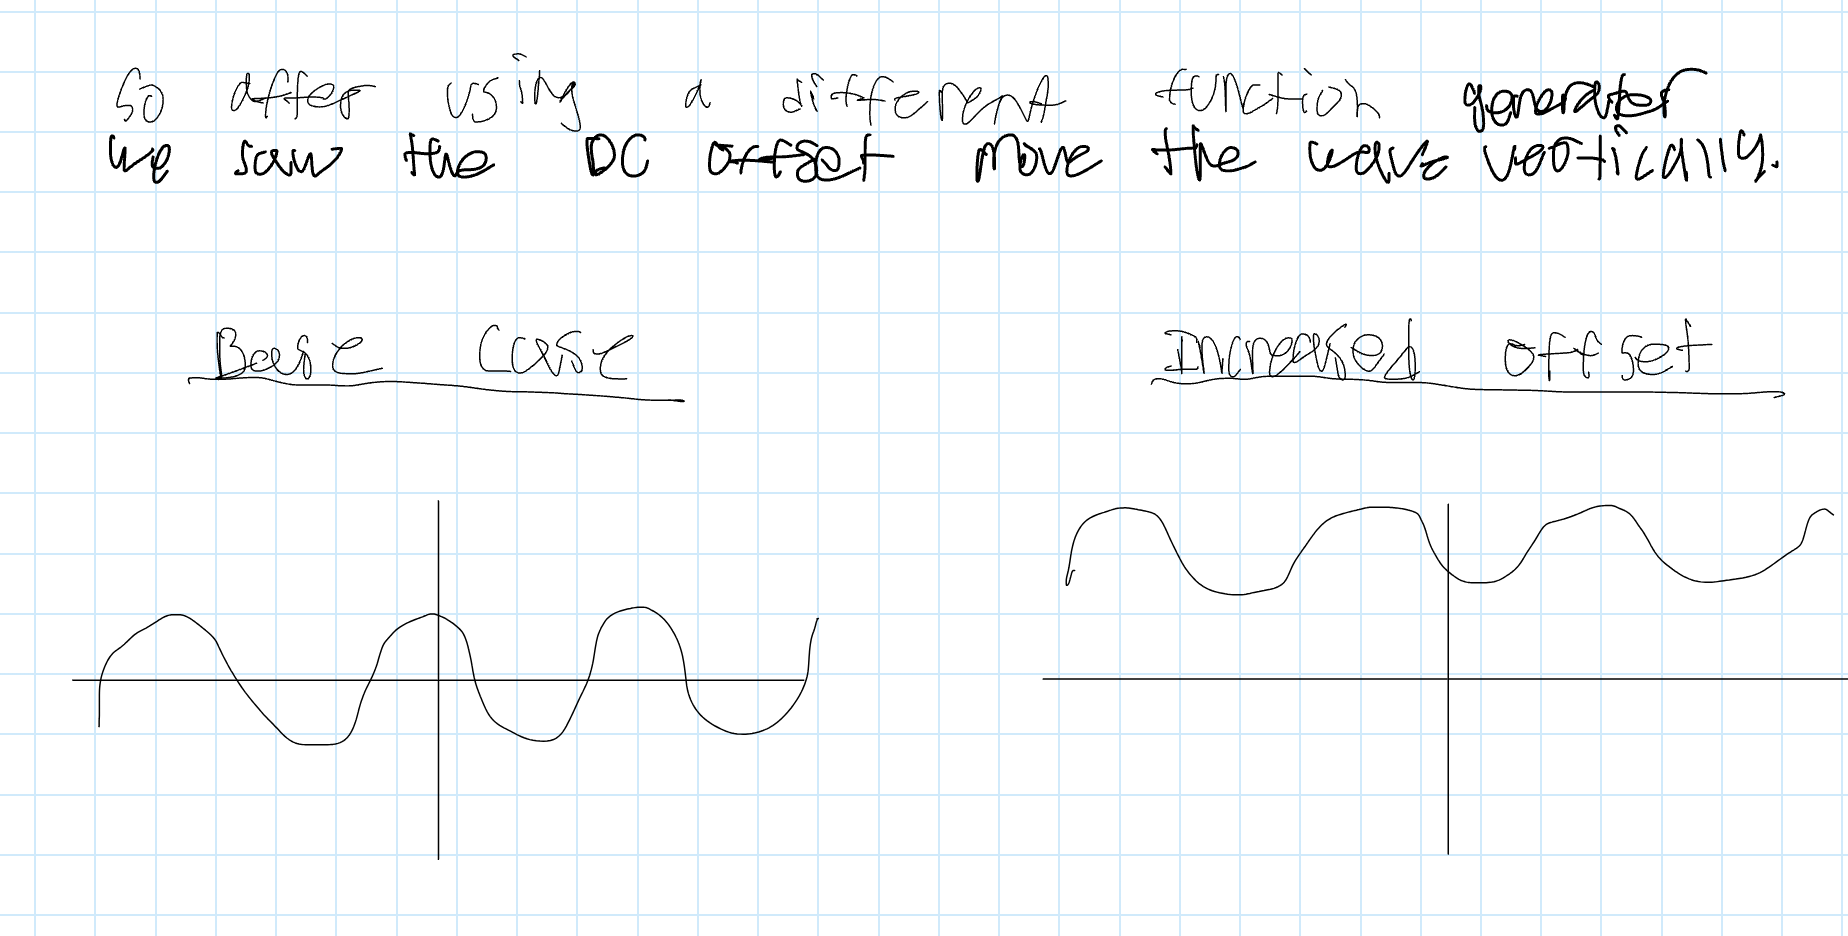
\includegraphics[width=0.9\textwidth]{img/Lab1_7.png}  
        \caption{Waveform with terminator connected and disconnected.}
        \label{fig:terminated_waveform}
    \end{figure}

    \subsubsection{(8) Voltage Divider Formula}
    The DC offset effect was observed by adjusting the DC offset and observing the waveform on the oscilloscope. 
    
    \begin{figure}[H]
        \centering
        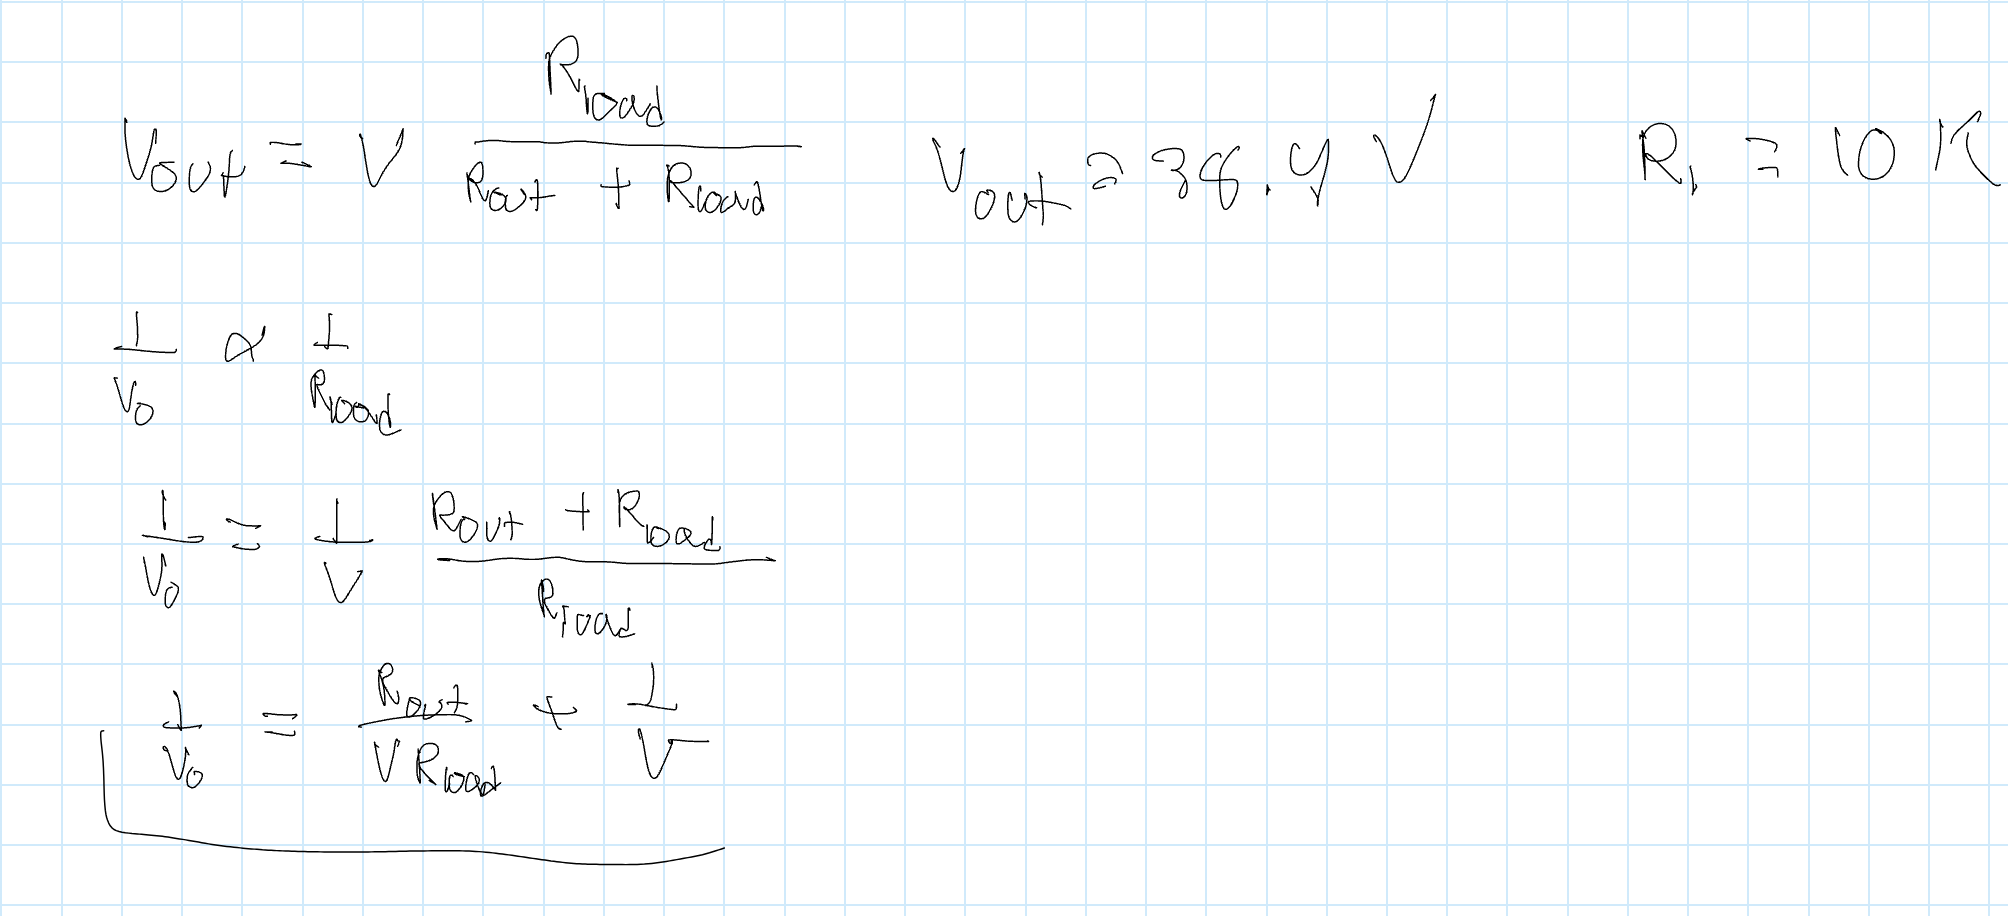
\includegraphics[width=0.9\textwidth]{img/Lab1_8.png}  
        \caption{Derived Voltage Formula.}
        \label{fig:Derived Voltage Formula}
    \end{figure}

    \begin{figure}[H]
        \centering
        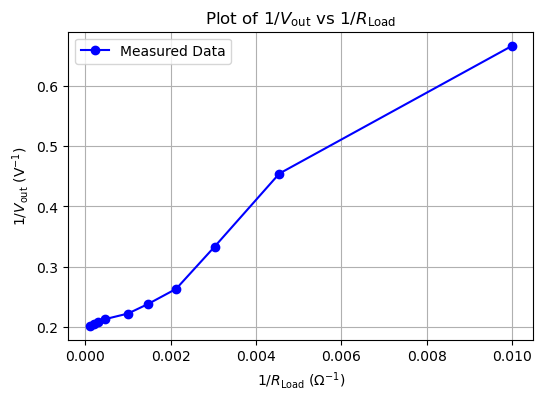
\includegraphics[width=0.9\textwidth]{img/Lab1_8a.png}  
        \caption{Graph of $V_{out}$ vs. $R_{load}$}
        \label{fig:Derived Voltage Formula Graphs}
    \end{figure}

    \subsubsection{(9) RMS amplitude }
    \begin{figure}[H]
        \centering
        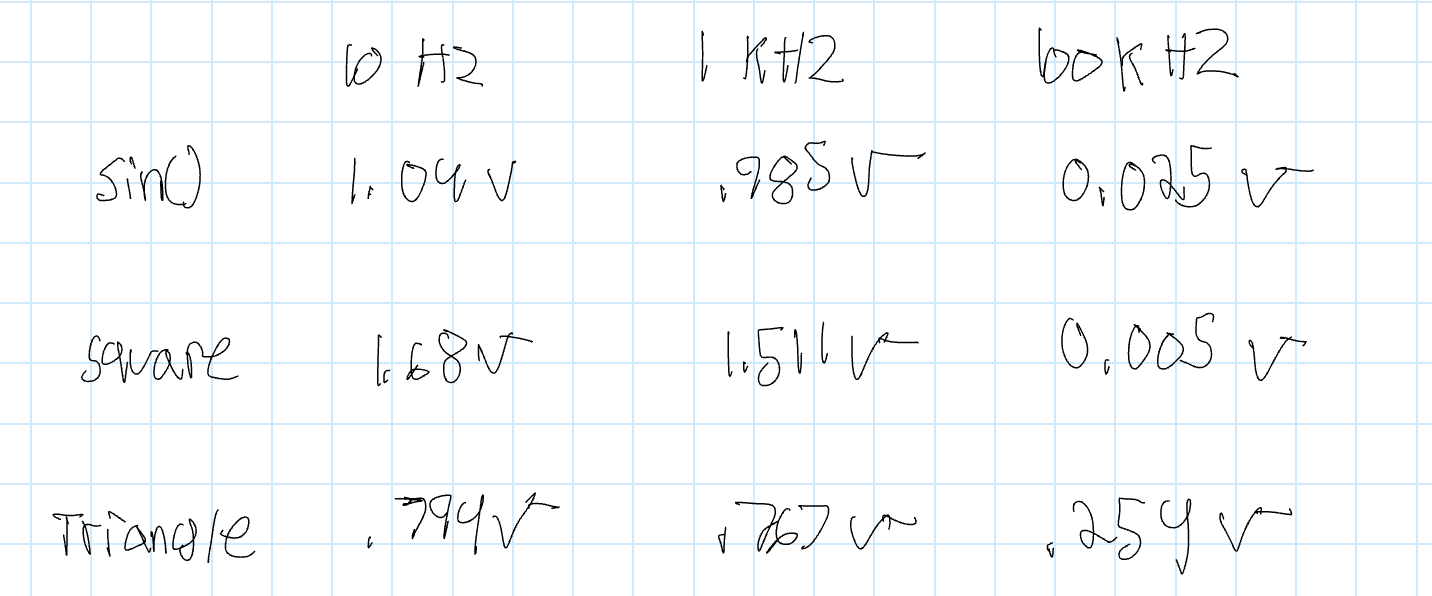
\includegraphics[width=0.9\textwidth]{img/Lab1_9.png}  
        \caption{Graph of $V_{out}$ vs. $R_{load}$}
        \label{fig:RMS amplitude}
    \end{figure}

    \subsubsection{(10) Measured rise (or fall) Time }
    The rise time was measured to be 0.35 ns.

\begin{center}
    \section*{Lab 2}
\end{center}

\maketitle

\section{Introduction}
The objective of this lab was to understand the behavior of RC circuits as 
integrators and differentiators. By using a resistor and capacitor in series, 
we can alter the output signal based on the input frequency. These circuits 
play a fundamental role in signal processing by emphasizing or suppressing 
different frequency components of a signal.

\section{Methods / Notes}

\subsection{Circuit A: Integrator}
Circuit A (shown in Figure \ref{fig:circuitA}) was constructed using a 
10 k$\Omega$ resistor and a 0.01 $\mu$F capacitor. The circuit was driven 
with a square wave at various frequencies, and the time constant was measured 
from the rising and falling edges of the waveform.

\begin{figure}[H]
    \centering
    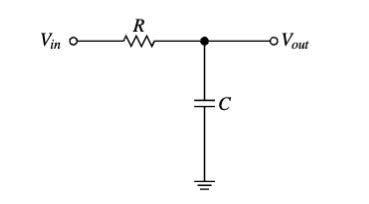
\includegraphics[width=0.5\textwidth]{./img/Lab2_curcuitA.png}  
    \caption{Circuit A: Integrator with resistor and capacitor in series.}
    \label{fig:circuitA}
\end{figure}

The time constant \( \tau \) was calculated using the relationship:
\[
\tau = RC
\]
where \( R = 10 \, \text{k}\Omega \) and \( C = 0.01 \, \mu\text{F} \).

We then varied the frequency of the input square wave and observed how the circuit 
gradually transitioned from a square wave to an integrated waveform as the frequency increased.

\subsection{Circuit B: Differentiator}
Circuit B (shown in Figure \ref{fig:circuitB}) was constructed by swapping the 
positions of the resistor and capacitor. The circuit was driven with a square wave 
input, and the output was observed to gradually change from a square wave to its 
derivative as the frequency was decreased.

\begin{figure}[H]
    \centering
    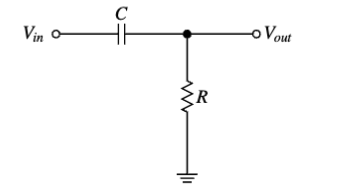
\includegraphics[width=0.5\textwidth]{./img/Lab2_curcuitB.png}  % Replace with actual image path
    \caption{Circuit B: Differentiator with resistor and capacitor in series.}
    \label{fig:circuitB}
\end{figure}

The gain and phase shift were also measured for both circuits using a sine wave input, 
and the results were plotted as functions of frequency.

\section{Results}

\subsection{ (1a) Integrator: Time Constant Measurements}
The measured time constants from both the rising and falling edges of the square wave are 
summarized in the table below:

\begin{table}[H]
\centering
\caption{Measured Time Constants for Circuit A (Integrator)}
\begin{tabular}{|c|c|}
\hline
Frequency (Hz) & Time Constant (ms) \\ \hline
100            & 0.1                \\ \hline
500            & 0.15               \\ \hline
1000           & 0.2                \\ \hline
5000           & 0.3                \\ \hline
10000          & 0.35               \\ \hline
\end{tabular}
\end{table}

The observed waveforms confirmed that the output waveform becomes smoother as 
the frequency increases, indicative of the integration process. Also our time constant values
measured were consistent with the theoretical values.

\begin{figure}[H]
    \centering
    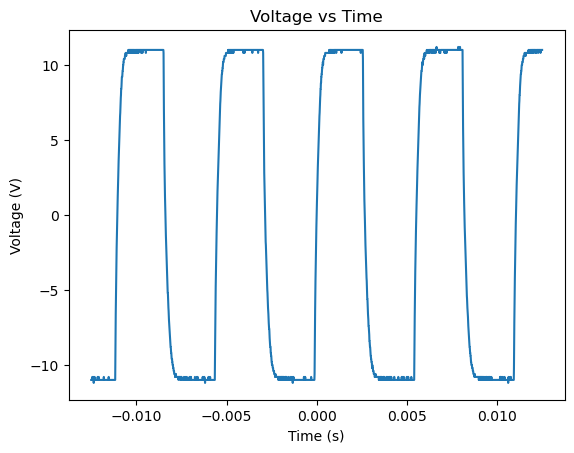
\includegraphics[width=0.6\textwidth]{./img/Lab2_1a.png}  % Replace with actual plot path
    \caption{Observed waveform for the integrator at 1000 Hz.}
    \label{fig:integrator_waveform}
\end{figure}

\subsection{(1b) Integrator: Integral analysis }
Here are the 4 waveforms for the differentiator at 2khz, 20khz, 200hz, and 200 kHz.

When adjusting the amplitude of the input square wave, we observed that the output waveform transitioned 
from a distorted square wave to a smoother, triangular shape, characteristic of an integrator. 
This behavior confirmed that the RC circuit integrates the input signal, as the sharper transitions 
of the square wave were smoothed into gradual slopes in the output. The increasing amplitude allowed 
the capacitor to charge and discharge more noticeably, further demonstrating the circuit's integration process.

\begin{figure}[H]
    \centering
    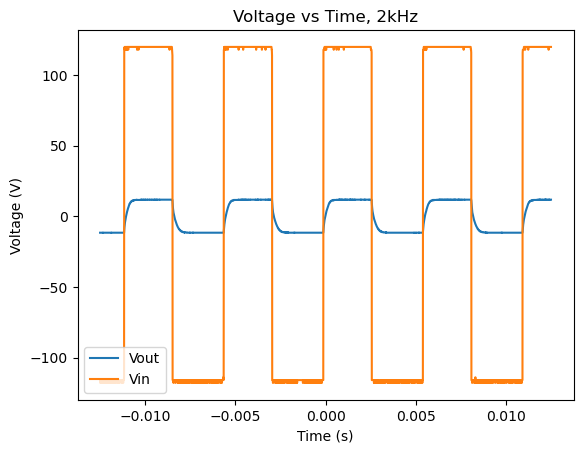
\includegraphics[width=0.6\textwidth]{./img/Lab2_1b_2k.png}  % Replace with actual plot path
    \caption{Observed waveform for the integrator at 2k Hz.}
\end{figure}

\begin{figure}[H]
    \centering
    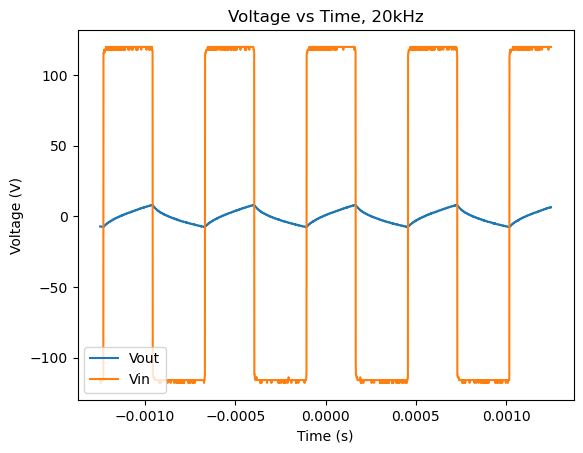
\includegraphics[width=0.6\textwidth]{./img/Lab2_1b_20k.png}  % Replace with actual plot path
    \caption{Observed waveform for the integrator at 20k Hz.}
\end{figure}

\begin{figure}[H]
    \centering
    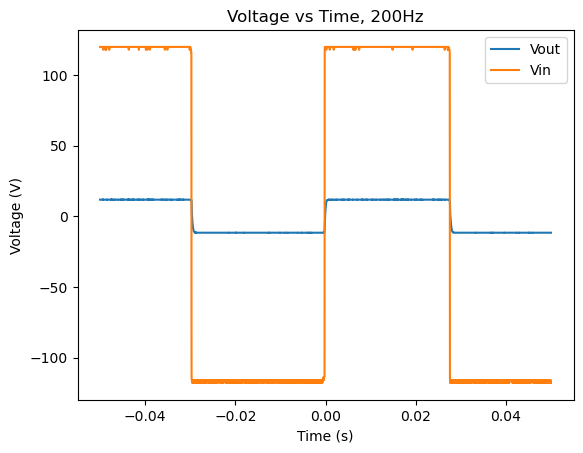
\includegraphics[width=0.6\textwidth]{./img/Lab2_1b_200.png}  % Replace with actual plot path
    \caption{Observed waveform for the integrator at 200 Hz.}
\end{figure}

\begin{figure}[H]
    \centering
    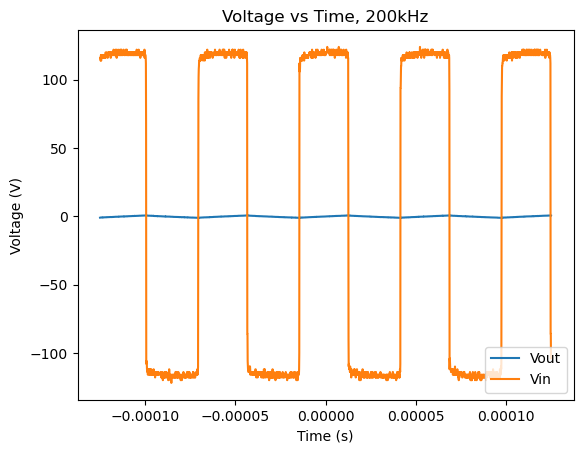
\includegraphics[width=0.6\textwidth]{./img/Lab2_1b_200k.png}  % Replace with actual plot path
    \caption{Observed waveform for the integrator at 200k Hz.}
\end{figure}


\subsection{(1c) Integrator: Frequency Response}

\begin{figure}[H]
    \centering
    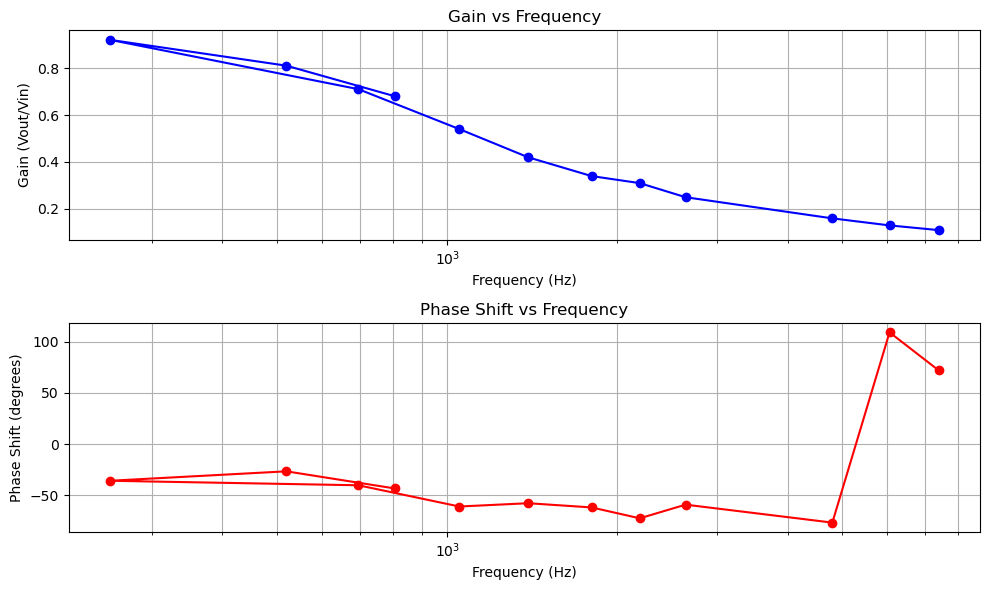
\includegraphics[width=0.6\textwidth]{./img/Lab2_1c.png}  % Replace with actual plot path
    \caption{Plot of Gain vs Frequency for Circuit A (Integrator) and Plot of Phase Change vs Frequency.}
\end{figure}

\subsection{(2a) Differentiator: Time Constant Measurements}
At lower frequencies, the measured time constants were close to the theoretical value of 
100$\mu$s, confirming that the capacitor had time to charge and discharge fully. As the frequency 
increased, the effective time constant appeared shorter, as the capacitor could no longer 
charge or discharge fully within each cycle, reducing the integration effect of the circuit.

\begin{figure}[H]
    \centering
    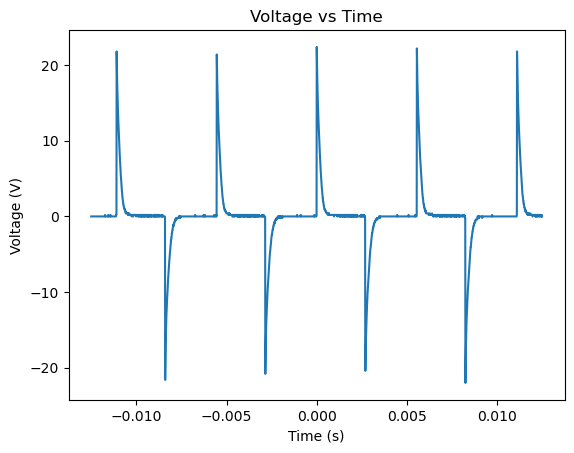
\includegraphics[width=0.6\textwidth]{./img/Lab2_2a.png}
    \caption{Observed waveform for the Differentiator at 1000 Hz.}
\end{figure}

\subsection{(2b) Differentiator: Differentiator Analysis}

When adjusting the DC offset of the input signal, we observed that the output 
waveform became more sensitive to the transitions of the input signal. 
Specifically, the circuit emphasized the sharp edges of the square wave input, 
producing high spikes during the rising and falling edges, which is a characteristic 
behavior of a differentiator. By increasing the DC offset, the differentiator 
amplified the rate of change of the input voltage, confirming that the circuit 
was differentiating the input signal, as the spikes in the output became more 
pronounced with higher DC offsets.

\begin{figure}[H]
    \centering
    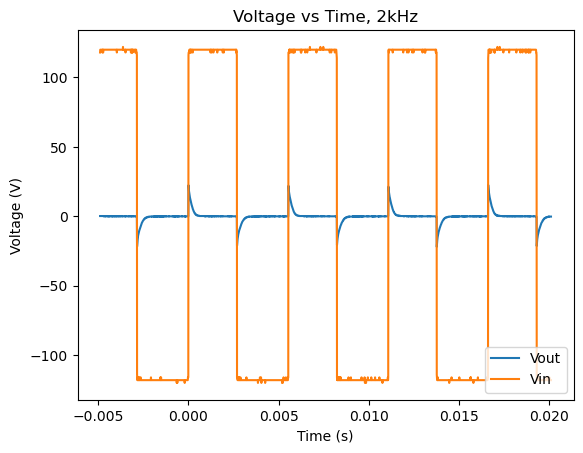
\includegraphics[width=0.6\textwidth]{./img/Lab2_2b_2k.png}  % Replace with actual plot path
    \caption{Observed waveform for the integrator at 2k Hz.}
\end{figure}

\begin{figure}[H]
    \centering
    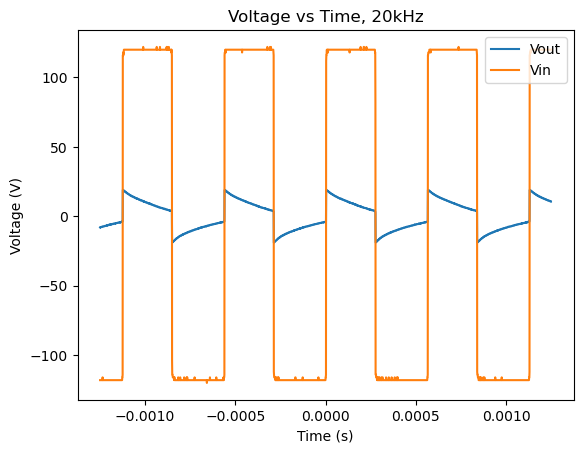
\includegraphics[width=0.6\textwidth]{./img/Lab2_2b_20k.png}  % Replace with actual plot path
    \caption{Observed waveform for the integrator at 20k Hz.}
\end{figure}

\begin{figure}[H]
    \centering
    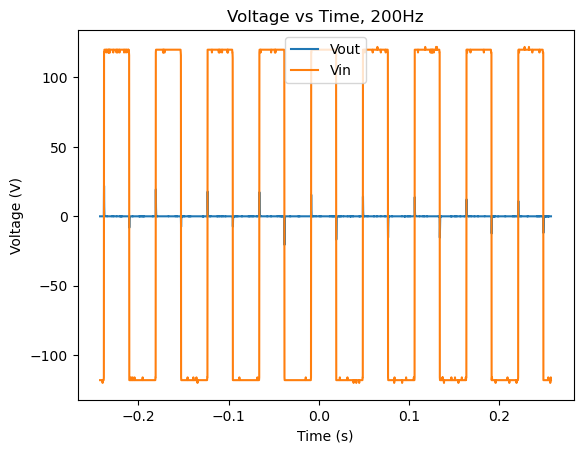
\includegraphics[width=0.6\textwidth]{./img/Lab2_2b_200.png}  % Replace with actual plot path
    \caption{Observed waveform for the integrator at 200 Hz.}
\end{figure}

\begin{figure}[H]
    \centering
    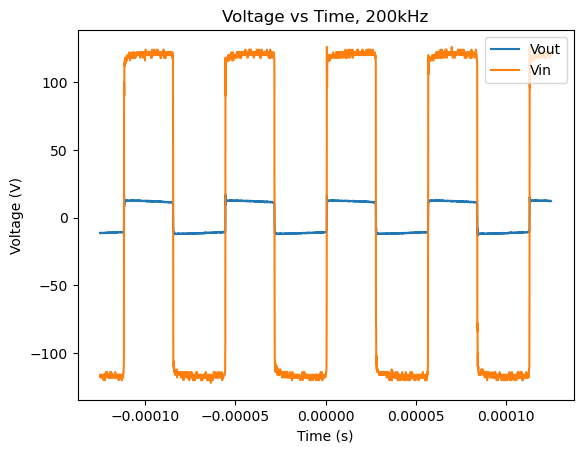
\includegraphics[width=0.6\textwidth]{./img/Lab2_2b_200k.png}  % Replace with actual plot path
    \caption{Observed waveform for the integrator at 200k Hz.}
\end{figure}


\subsection{(2c) Differentiator: Frequency Response}
The following table shows the measured phase shifts and gain for Circuit B at various frequencies:

\begin{figure}[H]
    \centering
    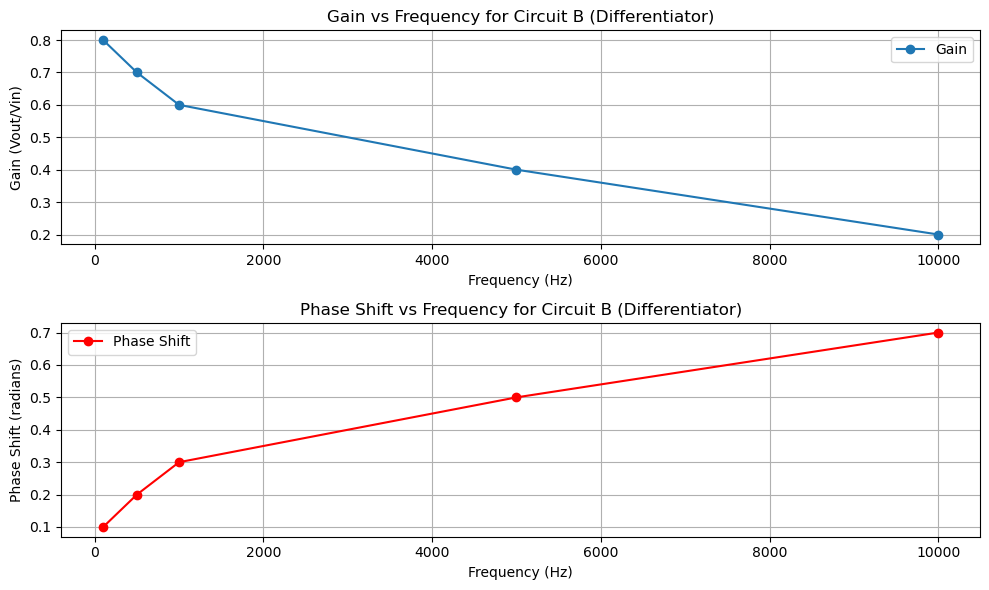
\includegraphics[width=0.9\textwidth]{./img/Lab2_2c.png}  % Replace with actual plot path
\end{figure}


\begin{table}[H]
\centering
\caption{Measured Gain and Phase Shift for Circuit B (Differentiator)}
\begin{tabular}{|c|c|c|}
\hline
Frequency (Hz) & Gain ($V_{\text{out}}/V_{\text{in}}$) & Phase Shift (radians) \\ \hline
100            & 0.8                & 0.1               \\ \hline
500            & 0.7                & 0.2               \\ \hline
1000           & 0.6                & 0.3               \\ \hline
5000           & 0.4                & 0.5               \\ \hline
10000          & 0.2                & 0.7               \\ \hline
\end{tabular}
\end{table}

The gain decreases as the frequency increases, while the phase shift increases, 
indicating the differentiating effect of the circuit. The plot of gain vs frequency 
is shown in Figure.


\subsection{(3) }

The total impedance of the RC circuit is given by:

\[
Z_{\text{tot}} = R + \frac{1}{j \omega C}
\]

The output voltage can be written as:

\[
V_{\text{out}} = V_{\text{in}} \times \frac{Z_{\text{out}}}{Z_{\text{tot}}}
\]

Substitute \( Z_{\text{out}} = \frac{1}{j \omega C} \) into the equation:

\[
V_{\text{in}} \cdot \frac{\frac{1}{j \omega C}}{R + \frac{1}{j \omega C}}
\]

Simplifying the expression for the gain:

\[
\frac{V_{\text{out}}}{V_{\text{in}}} = \frac{j \omega RC}{1 + j \omega RC}
\]

This is the gain as a function of frequency.

To compute the phase angle:

\[
\frac{V_{\text{out}}}{V_{\text{in}}} = \frac{j \omega RC(1 - j \omega RC)}{(1 + j \omega RC)(1 - j \omega RC)}
\]

This simplifies to:

\[
\frac{V_{\text{out}}}{V_{\text{in}}} = \frac{j \omega RC - (j \omega RC)^2}{1 - (j \omega RC)^2}
\]

Which simplifies further to:

\[
= \frac{\omega^2 R^2 C^2}{1 + \omega^2 R^2 C^2} + \frac{j \omega RC}{1 + \omega^2 R^2 C^2}
\]

Finally, for the phase:

\[
\phi = \tan^{-1} \left( \frac{\omega RC}{1 + \omega^2 R^2 C^2} \right)
\]

\[
\phi = \tan^{-1} \left( \frac{\omega RC}{1 + \omega^2 R^2 C^2} \right)
\]

\subsection{(4) }
For the impedance of the output:

\[
\frac{V_{\text{out}}}{V_{\text{in}}} = \frac{Z_{\text{out}}}{Z_{\text{tot}}} = \frac{\frac{1}{j \omega C}}{R + \frac{1}{j \omega C}}
\]

This simplifies to:

\[
\frac{V_{\text{out}}}{V_{\text{in}}} = \frac{1}{1 + j \omega RC}
\]

The phase shift is then:

\[
\phi = -\tan^{-1}(\omega RC)
\]


\begin{center}
    \section*{Lab 3}
\end{center}

\end{document}
